\let\negmedspace\undefined
\let\negthickspace\undefined
\documentclass[12pt, a4paper,twocolumn]{article}
\usepackage{geometry}
 \geometry{
 left=10mm,
 top=5mm,
 right=10mm,
 bottom=20mm,
 }
 \pagenumbering{gobble}
 \usepackage[utf8]{inputenc}
 \usepackage{graphicx}
 \usepackage{amsmath}
 \usepackage{amsfonts}
 \usepackage{amssymb}
 \usepackage{enumitem}
\usepackage{mathtools}
\usepackage[breaklinks=false]{hyperref}
\usepackage{listings}
\usepackage{calc}

\newcommand{\solution}{\noindent \textbf{Solution: }}
\newcommand{\question}{\noindent \textbf{Question: }}

\title{Assignment 1}
\author{Vishal Vijay Devadiga (CS21BTECH11061)}
\date{}
\begin{document}
% make the title area
\maketitle
\question
\begin{enumerate}[label=]
\item A(-1, 3), B(4,2) and C(3,-2) are the vertices of a triangle.
\begin{enumerate}
    \item Find the coordinates of the centroid G of the triangle
    \item Find the equation of the line through G and parallel to AC.
\end{enumerate}
\end{enumerate}
\solution
\begin{enumerate}
	\begin{figure}[htbp]
	\centerline{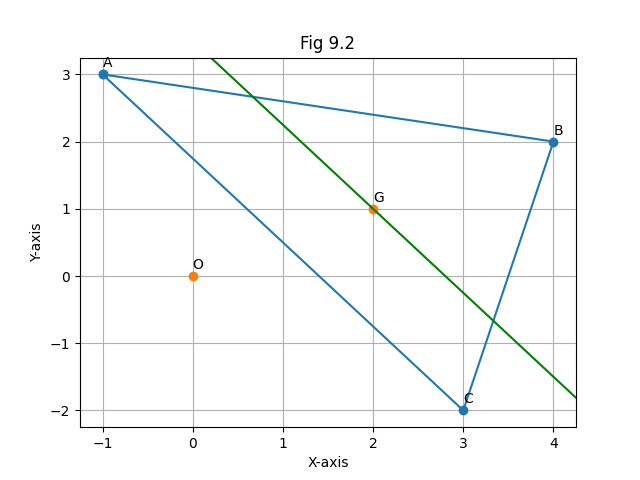
\includegraphics[scale = 0.6]{./figs/9.2.png}}
	\label{Figure 9.2}
	\end{figure}
\item Let $\vec{A}, \vec{B}, \vec{C}$ be the vectors OA,OB,OC respectively, where O is the origin.
	Thus,
	\begin{align*}
		\vec{A} = -\hat{i} + 3\hat{j} , 
		\vec{B} = 4\hat{i} + 2\hat{j} , 
		\vec{C} = 3\hat{i} - 2\hat{j}
	\end{align*}
	Using centroid formula,
    the desired point G is given by:
    \begin{align*}
        \vec{G}&= \frac{1}{3}(\vec{A} + \vec{B} + \vec{C})
        \\
        &= \frac{1}{3}(-\hat{i} + 3\hat{j} + 4\hat{i} + 2\hat{j} + 3\hat{i} - 2\hat{j})
        \\
        &=\frac{1}{3}(6\hat{i} + 3\hat{j})
        \\
        &= 2\hat{i} + \hat{j}
    \end{align*}
    G is the point $(2,1)$
\item Let L be the line that passes through G such that $L \parallel AC$
    Then, L can be expressed as $\vec{G} + k\hat{AC}$
    \begin{align*}
        \hat{AC} &= \frac{\vec{C} - \vec{A}}{\mid \vec{C} - \vec{A} \mid}
		\\        
        &= \frac{3\hat{i} - 2\hat{j} - (-\hat{i} + 3\hat{j})}{\mid 3\hat{i} - 2\hat{j} - (-\hat{i} + 3\hat{j}) \mid}
        \\
        &= \frac{4\hat{i} - 5\hat{j}}{\mid 4\hat{i} - 5\hat{j} \mid}
		\\        
        &= \frac{4\hat{i} - 5\hat{j}}{\sqrt{41}}
        \\
        L &= 2\hat{i} + \hat{j} + k(\frac{4\hat{i} - 5\hat{j}}{\sqrt{41}})
    \end{align*}
    Thus, Line L is $2\hat{i} + \hat{j} + m(4\hat{i} - 5\hat{j})$
\end{enumerate}
\end{document}